\documentclass[8pt,leqno]{beamer}

%%%%%%%%%%%%%%%%%%%%%%%% SET UP ENVIRONMENT ETC %%%%%%%%%%%%%%%%%%%%%%

\mode<presentation>
{
  \usetheme[]{} %Boadilla
% or ...
%	\useoutertheme[height=0pt,width=35pt]{sidebar}
%   \setbeamercolor{sidebar}{bg=gray!95!green}

  \setbeamercovered{transparent}
% or whatever (possibly just delete it)
}

\setbeamertemplate{navigation symbols}{}
%\usefonttheme[onlymath]{serif}
%\usefonttheme{professionalfonts}%[stillsansseriflarge]
\usepackage[english]{babel}
\usepackage[latin1]{inputenc}
\usepackage{fancybox}
%\usepackage{avant}
%\usepackage{cmbright}
\usepackage[T1]{fontenc}
\usepackage{fontawesome}
\usepackage{soul}
\setbeamercovered{dynamic}
\setbeamercolor{normal text}{fg=red!50!green!50!blue}
\setbeamercolor{alerted text}{fg=red!20!green!20!blue}


\setbeamercolor{structure}{fg=red!50!green!50!blue}

%\usepackage{fixpauseincludegraphics}
\usefonttheme{professionalfonts}
\usefonttheme{serif}
%\usepackage{fontspec}
%\setmainfont{Helvetica Neue}
\usepackage{times}
\usepackage{fontawesome}  % this package provides the Twitter logo, if needed
%\usecolortheme[RGB={100,100,150}]{structure}
%\setbeamertemplate{blocks}[rounded][shadow=true]
%\setbeamertemplate{background canvas}[vertical shading][bottom=black!10,top=white!100]
\usepackage{setspace}
%\usepackage{multimedia}
\usepackage{movie15}
\usepackage{pdfpages}
\usepackage{animate}
\usepackage{ifthen}
\usepackage{graphicx}


%%%%%%%%%%%%%%%%%%%%%%%% SET UP TITLE / AUTHORS ETC %%%%%%%%%%%%%%%%%%%%%%


\vspace*{0.75cm}
\title[\textcolor{gray}{\textbf{Modelling and data analysis `Winter School'}}] 
{\textcolor{white}{\Huge{Modelling and data analysis\\`Winter School'}}}

%
%\subtitle
%{} % (optional)

\vspace*{-0.125cm}
%\author[\textcolor{gray}{\faTwitter \hspace*{0.15cm} @nick\_golledge}] 
%{\textcolor{white}{\large{\faTwitter \hspace*{0.15cm} @nick\_golledge\inst{1}}\\\vspace*{0.0cm}
%
%\vspace*{0.125cm}
\author[\textcolor{gray}{}]{\textcolor{white}{Nick Golledge\inst{1}, \\
Liz Keller\inst{1,2},\\
Alex Gossart\inst{1},\\
Alena Malyarenko\inst{3},\\
Angela Bahamondes-Dominguez\inst{3},\\
Mario Krapp\inst{2},\\
Dan~Lowry\inst{2},\\
Stefan~Jendersie\inst{1}\\
%
%
}}


\normalsize
\institute[\textcolor{gray}{}] % (optional, but mostly needed)
{\textcolor{white}{
\inst{{1}}{Antarctic Research Centre, Victoria University of Wellington, New Zealand}\\
\inst{{2}}{GNS Science, Lower Hutt, New Zealand}\\
\inst{{3}}{NIWA, Wellington, New Zealand}\\
}


  \vspace*{1.2cm}


}
 
% - Use the \inst command only if there are several affiliations.
% - Keep it simple, no one is interested in your street address.

\date[\textcolor{gray}{}] % (optional)
{\vspace*{-4cm}


%%%%%%%%%%%%%%%%%%%%%%%% ADD SOME LOGOS %%%%%%%%%%%%%%%%%%%%%%


%\begin{columns}
%\column{2cm}
%\column{7cm}
\hspace*{-0.9cm} 
\includegraphics[height=1cm]{./logos/ASP_Hub_COL_black.png}\hspace*{0.2cm} 
\includegraphics[height=1cm]{./logos/VUW-logo-new.jpg}
\hspace*{0.0cm} 
\includegraphics[height=1cm]{./logos/mbie-logo.png} 
\hspace*{0.0cm} 
\includegraphics[height=1cm]{./logos/GNS_logo.jpg}
\hspace*{0.2cm} 
\includegraphics[height=1cm]{./logos/niwa-logo.png}
%\end{columns}
}

%%%%%%%%%%%%%%%%%%%%%%%% SET UP TEMPLATE HEAD / FOOT %%%%%%%%%%%%%%%%%%%%%%


\makeatletter
\setbeamertemplate{footline}
{
  \leavevmode%
  \hbox{%
  \begin{beamercolorbox}[wd=.333333\paperwidth,ht=2.25ex,dp=1ex,center]{author in head/foot}%
    \usebeamerfont{author in head/foot}\insertshortauthor~~\beamer@ifempty{\insertshortinstitute}{}{\insertshortinstitute}
  \end{beamercolorbox}%
  \begin{beamercolorbox}[wd=.333333\paperwidth,ht=2.25ex,dp=1ex,center]{title in head/foot}%
    \usebeamerfont{title in head/foot}\insertshorttitle
  \end{beamercolorbox}%
  \begin{beamercolorbox}[wd=.333333\paperwidth,ht=2.25ex,dp=1ex,right]{date in head/foot}%
    \usebeamerfont{date in head/foot}\insertshortdate{}\hspace*{2em}
    \insertframenumber{} / \inserttotalframenumber\hspace*{2ex} 
  \end{beamercolorbox}}%
  \vskip0pt%
}
\makeatother


\begin{document}

\newcommand{\movies}{off}


\setbeamercolor{background canvas}{bg=white}


%%%%%%%%%%%%%%%%%%%%%%%% SET BACKGROUND FOR TITLE SLIDE %%%%%%%%%%%%%%%%%%%%%%

\setbeamertemplate{background}{
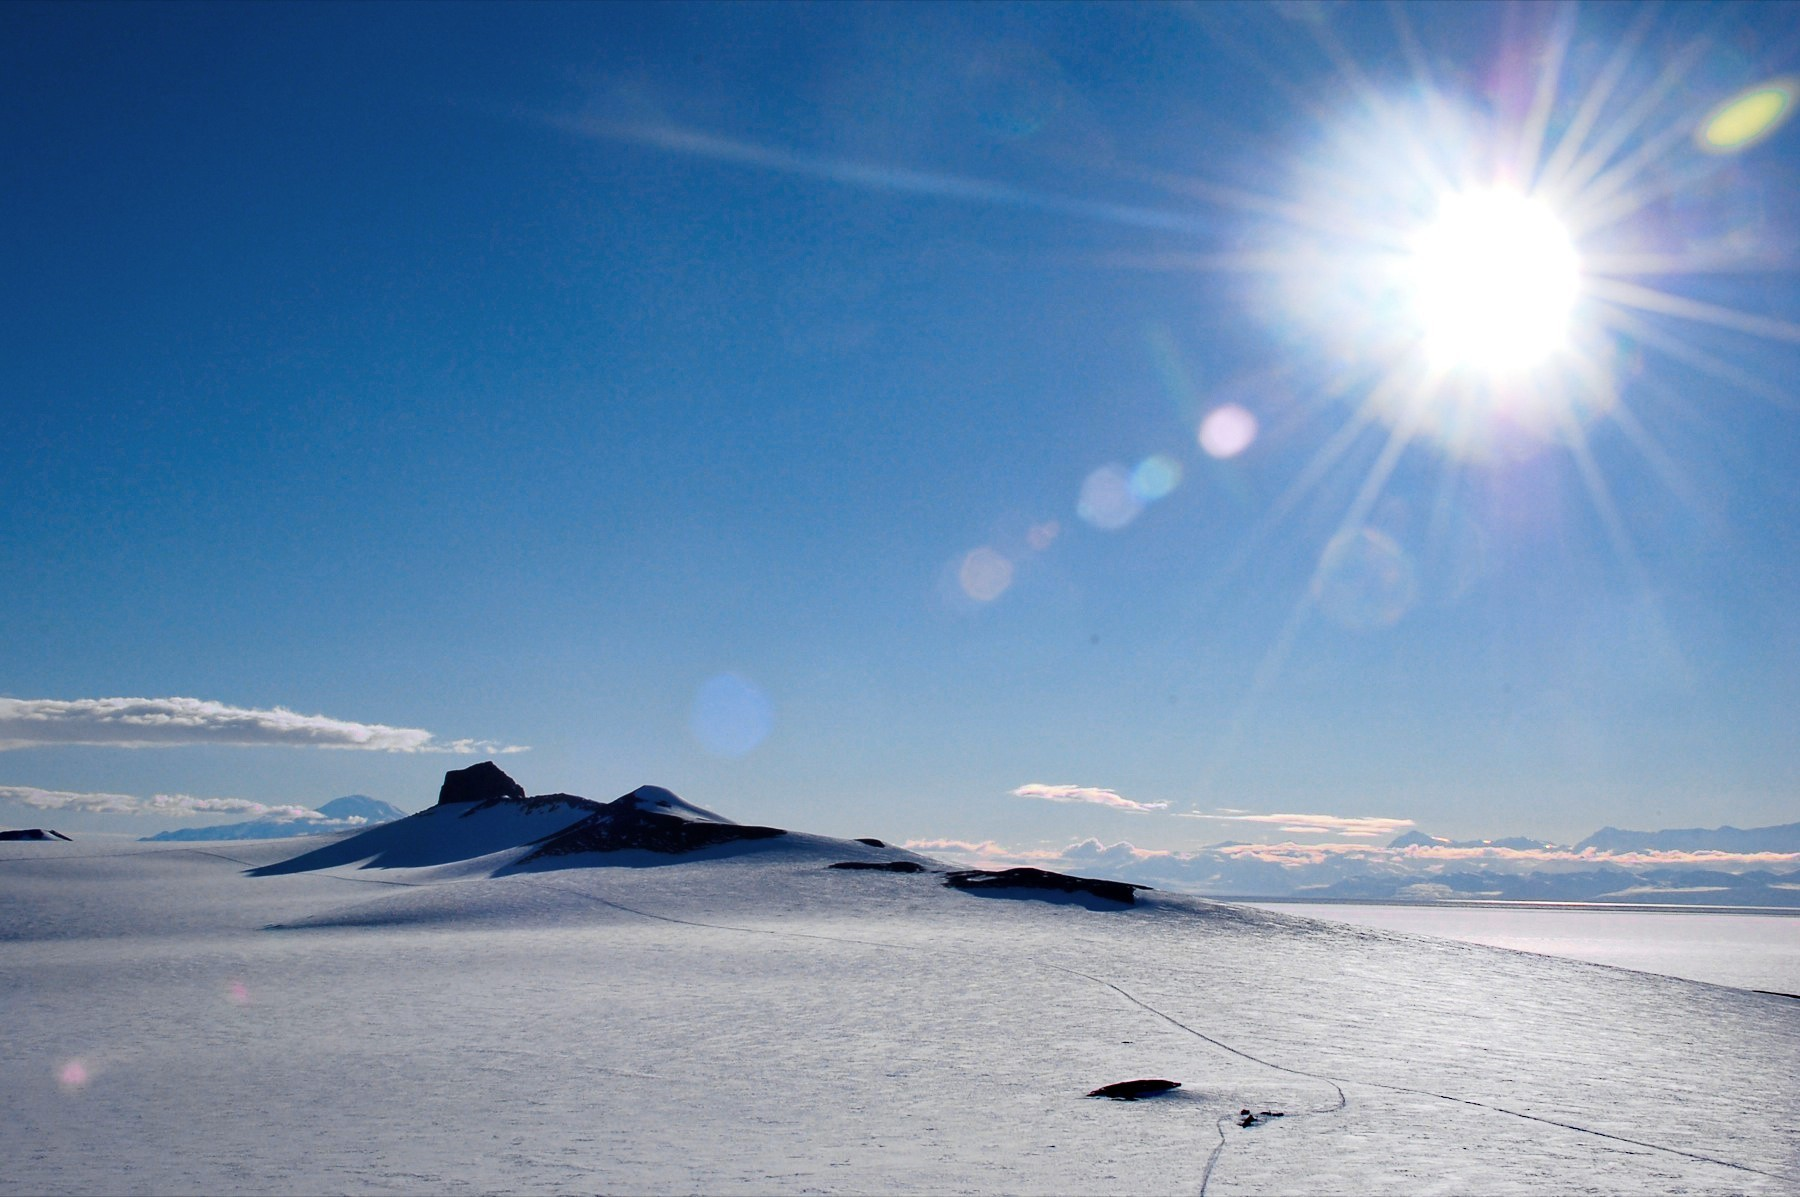
\includegraphics[width=\paperwidth,height=\paperheight]{./images/antarctic_4_tw.jpg}
}

\begin{frame}
  \titlepage
\end{frame}

%%%%%%%%%%%%%%%%%%%%%%%% CLEAR BACKGROUND FOR MAIN SLIDES %%%%%%%%%%%%%%%%%%%%%%

\setbeamertemplate{background}{}
\addtocounter{framenumber}{-1}

%%%%%%%%%%%%%%%%%%%%%%%% MAIN CONTENT %%%%%%%%%%%%%%%%%%%%%%




%%%%%%%%%%%%%%%%%%%%%%%% ADD CONTENT %%%%%%%%%%%%%%%%%%%%%%
\section{Intro}
\begin{frame}{\insertsectionnumber{ |} Welcome \& Introduction}

\textbf{Day 1} \\
\vspace*{0.75cm}\begin{tabular}{p{0.75cm}|p{7.5cm}|p{1.75cm}}
\hline 
10:00 & Arrival \& welcome & Nick \\
10:15 & Introduction to programming & Nick \\
& \small{Navigating the command line environment, scripting vs programming, pros \& cons of various languages} & \\
11:30 & Introduction to models & Liz \& Dan \\
& \small{Climate model basics: components, types of models, internal variability. CMIP overview, climate sensitivity} & \\
13:00 & Lunch &  \\
14:00 & Spatial data -- lecture & Alex \& Alena \\
& \small{Understanding gridded data, map projections, data analysis and manipulations, masking, extracting vertical / horizontal sections} & \\
15:30 & Coffee & \\
15:45 & Spatial data -- tutorial & Alex \& Alena \\
17:00 & Wrap-up & \\
\hline
\end{tabular}


\end{frame}

\begin{frame}{\insertsectionnumber{ |} Welcome \& Introduction}

\textbf{Day 2} \\
\vspace*{0.75cm}\begin{tabular}{p{0.75cm}|p{7.5cm}|p{1.75cm}}
\hline\\09:00 & Time-series data -- lecture & Mario \\
& \small{Principal component / empirical orthogonal function analysis, calculation of correlations, anomalies, detrending} & \\
10:30 & Coffee &  \\
10:45 & Time-series data -- tutorial & Mario \\
12:15 & Lunch & \\
13:15 & Document preparation in \LaTeX & Angela \\
& \small{Learn the basics, write equations, insert figures, create your own tables, insert references} & \\
14:45 & Afternoon tea &  \\
15:00 & Work Structure \& Version control & Stefan \\
& \small{Defining a workflow, handling `big data', version control for scripts/documents, best practice guidelines} & \\
\hline
\end{tabular}


\end{frame}

%%%%%%%%%%%%%%%%%%%%%%%%

\begin{frame}{\insertsectionnumber{ |} Aims, Methods, \& Scope}

\begin{columns}

\column[c]{7.5cm}

\begin{itemize}


\begin{beamerboxesrounded}[lower=gray,shadow=true]{\item The \textbf{aim} of the Winter School is that, by the end of the two days, participants will be able to find and download (climate model) data of interest, use simple scripts to process, analyse, and plot those data, integrate these outputs into a typeset document, and use version control software to keep track of changes.}\end{beamerboxesrounded}

\pause\begin{beamerboxesrounded}[lower=gray,shadow=true]{\vspace*{0.5cm}\item We will use \emph{\textbf{Python}} for the majority of the work but will incoporate examples from other languages if necessary. We'll introduce you to packages like \LaTeX ~and tools such as \emph{github}.}\end{beamerboxesrounded}

\pause\begin{beamerboxesrounded}[lower=gray,shadow=true]{\vspace*{0.5cm}\item This workshop is only intended to provide an \textbf{introduction} to working in a command-line environment, and exposure to some of the functionality available in this realm. It is not intended to be a complete course on programming, modelling, or data analysis ;-) }\end{beamerboxesrounded}


\end{itemize}

\end{columns}

\end{frame}


%%%%%%%%%%%%%%%%%%%%%%%% END CONTENT %%%%%%%%%%%%%%%%%%%%%%



%%%%%%%%%%%%%%%%%%%%%%%% END CONTENT %%%%%%%%%%%%%%%%%%%%%%


\end{document}